\subsection{Application: Intelligent Transportation and Autonomous Driving}

Autonomous-driving perception is a useful Foundations application because it exposes several ways in which an apparently simple benchmark comparison can become statistically invalid. Different datasets use different sensors, scene distributions, annotation policies, and metrics; different models may use camera, lidar, radar, maps, or sensor fusion; and deployment performance is affected by geography, weather, lighting, object rarity, and sensor degradation. A credible comparison therefore depends on matched protocols rather than on copying the highest score from a leaderboard.

The application also makes metric design concrete. A perception model must do more than classify objects: it must estimate position, size, orientation, velocity, and confidence well enough for downstream planning. The nuScenes Detection Score (NDS), for example, combines detection quality with multiple true-positive error terms. This illustrates a central Chapter 1 principle: the evaluation metric encodes the engineering objective, and choosing an incomplete metric can favor a model that is statistically strong but operationally weak.

The treatment here deliberately avoids reproducing the specialized architecture details developed later in the Computer Vision chapters. Instead, it focuses on dataset specification, modality-aware baseline comparison, distribution shift, error stratification, and deployment validation. The quantitative figure uses the Pass20 published nuScenes anchors and labels sensor modality explicitly so the reader can see why the bars are not a modality-controlled ranking.

\textbf{Problem}

The engineering task is to evaluate 3D perception models in a way that supports safe downstream planning. The benchmark must distinguish true improvements in perception from gains caused by additional sensors, external data, different test protocols, or incompatible evaluation metrics.

\textbf{Dataset}

Pass20 anchors the discussion in KITTI, nuScenes, Waymo Open Dataset, and Argoverse 2. KITTI provides a compact historical 2D/3D detection benchmark; nuScenes contains 1,000 multimodal driving scenes with cameras, radars, lidar, GPS, and IMU; Waymo provides large-scale perception segments; and Argoverse 2 emphasizes multimodal perception and motion forecasting with HD maps. These datasets should not be treated as interchangeable because their sensors, geography, annotations, and official metrics differ.

\textbf{Model}

The benchmark comparison includes a camera-only BEVFormer anchor, a lidar-based CenterPoint anchor, and a multimodal BEVFormer-M anchor. These systems represent different information budgets, so the comparison is useful for illustrating protocol and modality effects rather than for declaring one architecture universally superior.

\textbf{Method}

A reproducible experiment reports dataset version, split, sensor modalities, external data, backbone, training schedule, batch size, precision, random seeds, and the exact official evaluation script. Results from a validation split should not be mixed with test-server results, and camera-only methods should not be ranked against lidar or fusion methods without clearly identifying the modality difference.

\textbf{Evaluation}

Figure~\ref{fig:ch1-autonomous-driving-nds} plots the Pass20 nuScenes NDS anchors with sensor modality printed above each bar. Table~\ref{tab:ch1-autonomous-driving-benchmark} provides the same comparison in numerical form. NDS is used here because it reflects more than category detection, but deployment evaluation must also include class- and range-specific failures, latency, calibration, robustness, and closed-loop behavior.

\begin{figure}[t]
\centering
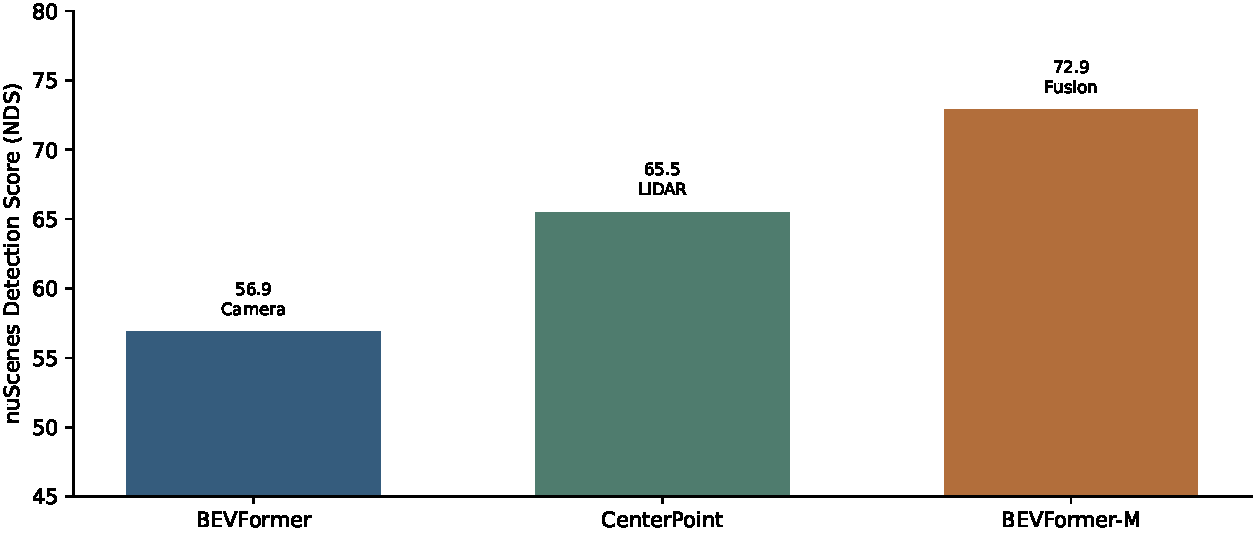
\includegraphics[width=\BookCompactFigureWidth]{figures/ch01_autonomous_driving_nds.pdf}
\caption{Published nuScenes detection anchors retained from Pass20. BEVFormer is camera-only, CenterPoint is lidar-based, and BEVFormer-M uses sensor fusion. The differing sensor modalities are shown explicitly because the NDS values are not a controlled architecture-only comparison. The figure is therefore used to teach protocol matching and confound control rather than to rank heterogeneous systems as if they consumed identical inputs.}
\label{fig:ch1-autonomous-driving-nds}
\end{figure}

\begin{table}[t]
\centering
\small
\caption{Published nuScenes benchmark anchors from the Pass20 evidence review. Sensor modality is part of the experimental condition and must be reported with the score.}
\label{tab:ch1-autonomous-driving-benchmark}
\begin{tabular}{llr}
\toprule
Method & Sensor modality & NDS \\
\midrule
BEVFormer & Camera & 56.9 \\
CenterPoint & LiDAR & 65.5 \\
BEVFormer-M & Fusion & 72.9 \\
\bottomrule
\end{tabular}
\end{table}

\textbf{Results}

The reported NDS values increase across the three anchors, but the input modality also changes from camera to lidar to fusion. The correct Chapter 1 interpretation is therefore not that the highest bar identifies the best architecture in isolation. Instead, the figure demonstrates why a benchmark claim must disclose the information available to each model and why a fair ablation must control the sensor configuration.

\textbf{Error Analysis}

Aggregate NDS can hide failures on distant pedestrians, occluded cyclists, rare vehicles, high-speed agents, nighttime scenes, adverse weather, unusual road geometry, or degraded sensors. Error analysis should therefore be stratified by class, range, occlusion, velocity, scene type, geography, and sensor health. Confidence calibration is also important because downstream planning decisions depend on uncertainty, not only on the predicted box coordinates.

\textbf{Limitations}

The table contains published benchmark anchors rather than a newly reproduced nuScenes training run, and the methods are not modality matched. It should therefore be read as an example of benchmark interpretation rather than a controlled causal comparison of architectures. Specialized detection, tracking, fusion, and closed-loop perception methods are developed in the later Computer Vision chapters.

\textbf{Deployment / Engineering Implications}

Offline benchmark performance is necessary but insufficient for an autonomous system. Candidate perception models require scenario replay, geographic holdouts, known-failure regression suites, sensor-dropout testing, latency measurements, calibration checks, shadow deployment, and rollback procedures. The Foundations lesson is that generalization and validation must be defined at the level of the operational system, not only at the level of a static test set.
